\section*{\centering Abstract}
Hamilton's equations are widely used in classical and quantum physics. The Hamiltonian Generative Network (HGN) is the first approach that aims to "learn the Hamiltonian dynamics of simple physical systems from high-dimensional observations without restrictive domain assumptions". To do so, a variational model is trained to reconstruct the evolution of physical systems directly from images by integrating the learned Hamiltonian. New trajectories can be sampled and rollouts can be performed forward and backward in time. In this work, we re-implement the HGN architecture and the physical environments (pendulum, body-spring system, and 2,3-bodies). We reproduce the paper experiments and we further expand them by testing on two new environments and one new integrator. Overall, we find that obtaining both good reconstruction and generative capabilities is hard and sensitive to the variational parameters.

\section*{\centering Reproducibility Summary}

\subsection*{Scope of Reproducibility}
The main objective of the paper is to "learn the Hamiltonian dynamics of simple physical systems from high-dimensional observations without restrictive domain assumptions".
To do so, the authors train a generative model that reconstructs an inputted sequence of images of the evolution of some physical system.
For instance, they learn the dynamics of a pendulum, a body-spring system, and 2,3-bodies.
In addition to these environments, we further expand the testing on two new environments and we explore architecture tweaks looking for performance gains.

\subsection*{Methodology}
We implement the project with Python using Pytorch \cite{pytorch} as a deep learning library.
Previous to ours, there was no public implementation of this work.
Thus, we had to write the code of the simulated environments, the deep models, and the training process.
The code can be found in this repository: \href{https://github.com/CampusAI/Hamiltonian-Generative-Networks}{https://github.com/CampusAI/Hamiltonian-Generative-Networks}
A single training takes around 4 hours and 1910MB of GPU memory (NVIDIA GeForce RTX2080Ti).


\subsection*{Results}
We found the model's input-output data slightly unclear in the original paper.
First, it seems that the model reconstructs the same sequence that has been inputted.
Nevertheless, further discussion with the authors seems to indicate that they input the first few frames to the network and reconstructed the rest of the rollout.
We test both approaches and analyze the results.
We generally obtain comparable results to those of the original authors when just reconstructing the input sequence ($30\%$ average absolute relative error w.r.t. to their reported values) and worse results when trying to reconstruct unseen frames ($107\%$ error).
In this report, we include our intuition on possible reasons that would explain these observations.


\subsection*{What was easy}
The architecture of the model and training procedure was easy to understand from the paper.
Besides, creating simulation environments similar to those of the original authors was also straightforward. 

\subsection*{What was difficult}
While the overall model architecture and data generation were easy to understand, we encountered the optimization to be especially tricky to perform.
In particular, finding a good balance between the reconstruction loss and KL divergence loss was challenging.
We implemented GECO \cite{geco} to dynamically adapt the Lagrange multiplier but it proved to be surprisingly brittle to its hyper-parameters, resulting in very unstable behavior.
We were unable to identify the cause of the problem and ended up training with simpler techniques such as using a fixed Lagrange multiplier as presented in \cite{beta-vae}.

\subsection*{Communication with original authors}
We exchanged around 6 emails with doubts and answers with the original authors.


\section{Introduction} \label{sec:intro}
\citet{zoubin2020} summarized the reasons for the success of deep learning in his talk given as the chief scientist in Uber. Firstly, with the availability of large datasets, large models can work well. Secondly, training such large models with stochastic descent works surprisingly well. Moreover, staying close to identity (such as ReLU) makes it stable to be trained. The automate differentiation and a large number of open source softwares make it scale well. Therefore, we can see deep learning in many applications, such as computer vision, natural language processing, bioinformatics, etc. 

However, it is not always the case where a huge number of labeled data are available. In some areas, it is difficult, expensive, or even impossible to have a large labeled dataset, such as medical images \citep{kuznetsova2018open}. In this case, it can be difficult to train a Deep Neural Network (DNN) from scratch with the limited labeled data. Luckily, \citet{tajbakhsh2016convolutional} shows that a DNN trained based on a pre-trained DNN, fine-tuning, can outperform the one trained from scratch. Moreover, Semi-Supervised Learning (SSL) is also a common method to deal with the scarcity and often high acquisition cost of labelled data \citep{pmlr-v124-kugelgen20a}. SSL efficiently leverages labeled data and the relation with unlabeled data to train a DNN.
% Interestingly, among SSL methods, there is a class of methods of which names contain "Match", 
Among SSL methods, there is a class of "match"-based methods,
such as FixMatch \citep{sohn2020fixmatch}, MixMatch \citep{berthelot2019mixmatch}, ReMixMatch \citep{kurakin2020remixmatch} and DivideMatch \citep{li2020dividemix}. These methods utilize the consistency regularization, pseudo-labelling and ensembling methods to boost the performance with the use of unlabeled data. In fact, they are leveraging prior knowledge to regularize the training of DNNs.
In this project, we focus on reproducing and investigating one of such methods, FixMatch \citep{sohn2020fixmatch}.

Nevertheless, SSL is still facing many challenges in theory and in practice. \citet{ben2008does} show that “as long as one does not make any assumptions about the behavior of the
labels, SSL cannot help much over algorithms that ignore
the unlabeled data.” Moreover, SSL can actually degrade performance if certain assumptions are not met \citep{chapelle2010semi}. In this line of works, \citet{scholkopf2012causal} consider the problem from a causal modeling perspective and conclude that in fact SSL is impossible when predicting a target variable from its causes (causal learning) but possible from anti-causal learning. Recently, the relation of causality and semi-supervised learning is further explored in \citep{pmlr-v124-kugelgen20a}, i.e., predicting a target variable from both causes and effects at the same time. Moreover, in the light of consistency regularization and pseudo-labelling, a significant issue of the "Match"-based methods is \textit{confirmation error}. 
It happens especially when noisy samples are in the labeled set. A DNN can keep having lower loss by fitting the noise and be further maintained after training with the wrong pseudo labels of unlabeled data , which keeps the errors in the model and limits its generalization and performance \citep{tarvainenweight}. This problem becomes more serious in the presence of asymmetric noise in the training labels, which roughly speaking tends to label a class of data as another specific class. 

Therefore, in this work, we are not only reimplementing FixMatch, but also investigating whether the pseudo labels made by the DNN contain harmful noise leading to confirmation errors. 
First, we design a stable and reliable method to examine the existence of confirmation errors and noisy pseudo labels by reconstructing the batch structure.
Secondly, we find methods to deal with (asymmetric) noise in (pseudo) labels of the training dataset. 
We reconstruct the batch structure and add an equal-frequency entropy regularization on labeled data to the loss function of FixMatch. 
Moreover, we also use a confidence entropy regularization on labeled data to avoid the over-confident prediction. 
It turns out that both entropy regularization is helpful for dealing with the noisy (pseudo) labels (even for the asymmetric noise) and confirmation errors.
% Finally, we manually add asymmetric noise in the labeled data and compare the performance of baseline FixMatch, FixMathc with equal-frequency entropy regularization and FixMatch with the confidence entropy regularization.
Our experimental results show that \\
\begin{enumerate}
\vspace{-0.5cm}
    \item our implementation can achieve almost the same performance even better for low-label regimes.
    \item there exists asymmetric noise in the pseudo labels leading to confirmation errors. With such pseudo labels, the model is biased which in turn leads to more asymmetric noise in pseudo labels.
    \item FixMatch with equal-frequency entropy regularization and FixMatch with confidence entropy regularization can reduce (asymmetric) noise in the pseudo labels and perform better than the baseline FixMatch in the presence of asymmetric noise in (pseudo) labels .
\end{enumerate}


\section{Scope of reproducibility}
\label{sec:claims}

In order to verify the central claims presented in the paper we focus on the following target questions:

\begin{itemize}
    \item Does \textit{RigL} outperform existing sparse-to-sparse training techniques---such as SET (\citet{Mocanu2018SET}) and SNFS (\citet{dettmers2020sparse})---and match the accuracy of dense-to-sparse training methods such as iterative pruning (\citet{to_prune_or_not})?
    
    \item \textit{RigL} requires two additional hyperparameters to tune. We investigate the sensitivity of final performance to these hyperparameters across a variety of target sparsities (Section \ref{hyperparameter-tuning}).
    
    \item How does the choice of sparsity initialization affect the final performance for a fixed parameter count and a fixed training budget (Section \ref{effect-sparsity-distribution})?
    
    \item Does redistributing layer-wise sparsity during connection updates (\citet{dettmers2020sparse}) improve \textit{RigL}'s performance? Can the final layer-wise distribution serve as a good sparsity initialization scheme (Section \ref{effect-redistribution})? 

\end{itemize}

\section{Methodology}

We have re-implemented the algorithm proposed in the paper from scratch using PyTorch and created an end-to-end model trainer with a Keras-like interface. We referred to the code given by the authors for the baseline model hyperparameters and the source of synthetic datasets. The algorithm presented by the original authors in their paper can be represented as follows:

\begin{algorithm}[H]
\SetAlgoLined
\DontPrintSemicolon

\KwInput{\textbf{Input:} Initialize $\lambda$} \;

\For{number of training epochs}{
    \For{ i = 1,...,number of mini-batch examples}{
        Sample $ \epsilon \sim \mathcal{U}(0,1) $ and set $\delta = \frac{1}{2}\log\frac{\epsilon}{1-\epsilon}$ \;
        Initialize $w_{b}$ = $\tanh((\lambda + \delta)/\tau)$ \;
        Compute following using \textit{gumbel-softmax} trick \[ g_i :=  \frac{1}{M} \nabla_{w_{b}}l(y_{i}, f_{w_{r}}(x_{i})) \] \[s_i := \frac{N(1-w^2_{b})}{\tau(1-\tanh(\lambda)^2)}\]
    }
    Update $\mu$ and $\lambda$ using following equation \[\mu \leftarrow \tanh(\lambda) \] \[\lambda \leftarrow (1-\alpha)\lambda - \alpha[\sum\limits_{i=1}^{M} (s_i\odot g_i) - \lambda_{0}]\]
}
\caption{Bayesian Learning rule for BayesBiNN}
\label{alg:alg1}
\end{algorithm}

This would make the paper easier to interpret and this implementation on code.
Some of the mathematical expressions mentioned in the original paper were presented from various sources and missed out several intermediate steps which we found to be very important while reproducing the paper from scratch. Here we present a step-wise derivation of some important expressions written in the original paper: 

Bayesian formulation of the discrete optimization problem, in which loss has to be minimized w.r.t posterior $q(w)$, given prior $p(w)$ can be written as: 
\[\mathbb{E}_{q(\,w)\,} [\,\sum\limits_{i=1}^{N}l(\,y_{i}, f_{w}(\,x_{i})\,)\,]\, + \mathcal{D}_{KL}[\,q(w)\|p(w)]\,\]
To solve the above optimization problem, Bayesian learning rule given in \citet{r6} is applied, assuming solution to be a part of minimal exponential family of distribution, given by: \[q(w) = h(w)\text{exp}[\lambda^{T}\phi(w) - A(\lambda)]\]  
where base measure $h(w)$ is assumed to be 1. Following is the update rule used to learn $\lambda$: \[\lambda \leftarrow (1-\rho)\lambda - \rho[\nabla_{\mu}\mathbf{E}_{q(w)}[l(y_{i} f_{w}(x_{i}))]-\lambda_{0}]\] where $\rho$ is the learning rate, $\mu = \mathbf{E}_{q(w)}[\phi(w)]$. Bernoulli distribution being a special case of minimal exponential family distribution, we assume prior $p(w) \sim \mathrm{Bern}(p)$ with $p = 0.5$, and posterior $q(w)$ to be mean-field Bernoulli distribution: \[q(w) = \prod_{j=1}^W p_{j}^{\frac{1+w_{j}}{2}}(1-p_{j})^{\frac{1-w_{j}}{2}} \]   

For weight $j$, \[q(w_j) = \mathrm{exp}(\frac{1}{2}(1+w_j)\log p_j + \frac{1}{2}(1-w_j)\log(1-p_j))\] \[ = \mathrm{exp}(\underbrace{w_j}_{\phi(w)}\underbrace{\frac{1}{2}\log\frac{p}{1-p})}_{\lambda} + \frac{1}{2}\log(p(1-p))\]
Comparing above expression with minimal exponential family distribution, we can say:
\[\lambda = \frac{1}{2}\log\frac{p}{1-p} \, \mathrm{and} \, \phi(w) = w.\]

We defined $\mu = \mathbb{E}_{q(w)}[\phi(w)]$,
\[\mu = \int wq(w)dw = \mathbb{E}[q(w)] = \sum\limits_{w^{i}\in\{-1,1\}}w^{i} q(w^{i}) \] \[= \sum\limits_{w^{i}\in\{-1,1\}}w^{i} p^{\frac{1+w^{i}}{2}}(1-p)^{\frac{1-w^{i}}{2}} = -(1-p) + p\]
\[= 2p-1\]
From above derivations we can say that, $p = 1/(1 + \mathrm{exp}(-2\lambda)) = \mathrm{Sigmoid}(2\lambda)$ and $q(w) \sim \mathrm{Bern}(p)$.

To implement the update rule, we need to compute the gradient with respect to $\mu$. Original paper uses a reparamaterization trick called  gumbel-softmax trick \citet{r7}, which is used to relax the discrete random variables of a concrete distribution (for eg, bernoulli distribution).  Binary concrete relaxation \citet{r7} of binary concrete random variable $X \in (0,1)$ with distribution $X \sim \mathrm{BinConcrete}(\alpha, \lambda)$ with temperature $\lambda$ and location $\alpha $, \[X = \frac{1}{1 + \mathrm{exp}(-(\log\alpha + L)/\lambda)}\] where $L \sim $ Logistic. And its density is given by \[p_{\alpha,\lambda}(x) = \frac{\lambda\alpha x^{-\lambda-1}(1-x)^{-\lambda-1}}{(\alpha x^{-\lambda} + (1-x)^{-\lambda})^{2}}\]

Using above expressions, for binary weights $w_j \in \{0,1\}$, relaxed variable $w_{r}^{\epsilon_{j}, \tau}(p_j) \in (0,1)$ can be used with temperature $\tau$ and $\alpha = e^{2\lambda}$ given by \[ w_{r}^{\epsilon_{j}, \tau}(p_j) = \frac{1}{1 + \mathrm{exp}(-\frac{2\lambda_j + 2\delta_j}{\tau})},\] where $\delta_j \sim$ Logistic and its density is given by \[p(w_{r}^{\epsilon_{j}, \tau}(p_j)) = \frac{\tau e^{2\lambda} w_{r}^{\epsilon_{j}, \tau}(p_j)^{-\tau-1}(1-w_{r}^{\epsilon_{j}, \tau}(p_j))^{-\tau-1}}{(e^{2\lambda} w_{r}^{\epsilon_{j}, \tau}(p_j)^{-\tau} + (1-w_{r}^{\epsilon_{j}, \tau}(p_j))^{-\tau})^{2}}\]

% Start with a high-level overview of your results. Does your work support the claims you listed in section 2.1? Keep this section as factual and precise as possible, reserve your judgement and discussion points for the next "Discussion" section. 

% Go into each individual result you have, say how it relates to one of the claims and explain what your result is. Logically group related results into sections. Clearly state if you have gone beyond the original paper to run additional experiments and how they relate to the original claims. 

% \subsection{Result 1}

% \subsection{Result 2}

% \subsection{Additional results not present in the original paper}

\section{Results} \label{sec:reproduction}

We first test whether the HGN \cite{hgn} can learn the dynamics of the four presented physical systems by measuring the average mean squared error (MSE) of the pixel reconstructions of each predicted frame.
Furthermore, we test the original HGN architecture along with different modifications: a version trained with Euler integration rather than Leapfrog integration (HGN Euler),
%a version trained with no transformer network (HGN no $f_\psi$),
and a version that does not include sampling from the posterior $q_\phi(\bm{z}|\bm{x}_0 ... \bm{x}_T)$ (HGN determ). Since we could not find suitable GECO\cite{geco} hyperparameters, we use a fixed Lagrange multiplier\cite{beta-vae} in all the experiments.
%To test HNN, we use the implementation provided by \cite{hnn} known as pixelHNN.
%Similarly to \cite{hgn}, we test HNN with a modification of the architecture to closely match the HGN (HNN Conv).

\begin{table}[]
    \centering
    \resizebox{\textwidth}{!}{%
    \begin{tabular}{c c c c c c c c c}
     \Xhline{3\arrayrulewidth}
     \textsc{Model} & \multicolumn{2}{c}{\textsc{Mass-spring}} & \multicolumn{2}{c}{\textsc{Pendulum}} & \multicolumn{2}{c}{\textsc{Two-body}} & \multicolumn{2}{c}{\textsc{Three-body}} \\
     & \textsc{Train} & \textsc{Test} & \textsc{Train} & \textsc{Test}& \textsc{Train} & \textsc{Test}& \textsc{Train} & \textsc{Test}\\
    \Xhline{3\arrayrulewidth}
     
    Orig. \textsc{HGN (Euler)} \cite{hgn} & $3.67 \pm 1.09$ & $6.2 \pm 2.69$ & $5.43 \pm 2.53$ & $10.93 \pm 4.32$ & $6.62 \pm 3.93$ & $15.06 \pm 7.01$ & $7.51 \pm 3.49$ & $9.4 \pm 3.92$ \\
    Orig. \textsc{HGN (Determ)} \cite{hgn} & $0.23 \pm 0.23$ & $3.07 \pm 1.06$ & $0.79 \pm 1.24$ & $10.68 \pm 3.19$ & $2.34 \pm 2.3$ & $14.47 \pm 5.24$ & $4.1 \pm 2.05$ & $5.17 \pm 1.96$ \\
    %Orig. \textsc{HGN (No $f_\psi$)} \cite{hgn} & $4.95 \pm 1.71$ & $7.04 \pm 2.55$ & $6.83 \pm 3.29$ & $13.98 \pm 4.94$ & $6.35 \pm 3.86$ & $16.49 \pm 6.6$ & $8.37 \pm 3.13$ & $10.41 \pm 3.72$ \\
    Orig. \textsc{HGN (Leapfrog)} \cite{hgn} & $3.84 \pm 1.07$ & $6.23 \pm 2.03$ & $4.9 \pm 1.86$ & $11.72 \pm 4.14$ & $6.36 \pm 3.29$ & $16.47 \pm 7.15$ & $7.88 \pm 3.55$ & $9.8 \pm 3.72$ \\
     \Xhline{3\arrayrulewidth}
     \textsc{HGN (Euler)} ours & $9.05 \pm 0.02$ & $9.06 \pm 0.05$ & $17.79 \pm 0.06$ & $17.86 \pm 0.13$ & $3.84 \pm 0.01$ & $3.85 \pm 0.02$ & $1.99 \pm 0.01$ & $1.99 \pm 0.01$ \\
     \textsc{HGN (Determ)} ours & $7.10 \pm 0.01$ & $7.10 \pm 0.03$ & $14.11 \pm 0.05$ & $14.14 \pm 0.12$ & $3.92 \pm 0.02$ & $3.93 \pm 0.02$ & $4.14 \pm 0.01$ & $4.13 \pm 0.02$ \\

     \textsc{HGN (Leapfrog)} ours & $7.11 \pm 0.01$ & $7.12 \pm 0.03$ & $14.89 \pm 0.05$ & $14.97 \pm 0.1$ & $3.36 \pm 0.01$ & $3.36 \pm 0.02$ & $8.81 \pm 0.01$ & $8.81 \pm 0.01$ \\
     \Xhline{3\arrayrulewidth}
     \textsc{HGN (Euler)} ours \textit{5-frame inference} & $42.09\pm 0.14$ & $41.98\pm 0.32$ & $47.06\pm 0.17$ & $47.03\pm 0.39$ & $6.46\pm 0.03$ & $6.52 \pm 0.06$ & $8.18 \pm 0.01$ & $8.17 \pm 0.01$ \\
     \textsc{HGN (Determ)} ours \textit{5-frame inference}& $13.00 \pm 0.05$ & $13.04 \pm 0.11$ & $45.06\pm 0.19$ & $44.89 \pm 0.42$ & $10.95\pm 0.02$ & $10.97 \pm 0.05$ & $3.72\pm 0.01$ & $3.72\pm 0.02$ \\
     \textsc{HGN (Leapfrog)} ours \textit{5-frame inference}& $12.15 \pm 0.05$ & $12.21 \pm 0.11$ & $44.29\pm 0.19$ & $44.12\pm 0.42$ & $6.28 \pm 0.03$ & $6.33 \pm 0.06$ & $3.35\pm 0.01$ & $3.35\pm 0.02$ \\
     \Xhline{3\arrayrulewidth}
    
    \end{tabular}}
    \vspace{0.25cm}
    \caption{Average pixel MSE of the reconstruction of a 30-frame rollout sequence on the test and train datasets of the four physical systems presented by \cite{hgn}. All the values are multiplied by $10^4$. We show our results (second and third group) along with the ones reported by the original authors (first group). In the second group, we train to reconstruct the whole inputted sequence (as an autoencoder) and in the third group, we train by inputting only the first 5 frames.}
    \label{tab:reproduction}
\end{table}

Table \ref{tab:reproduction} shows the results of the experiments described previously along with the results of the original authors. As it can be seen, we achieve average pixel reconstruction errors that are similar (30\% avg absolute error w.r.t. the reported values on the test set using Leapfrog integrator) to the ones reported in the original paper when reconstructing the same sequence that is inputted (we call this version \textit{autoencode}).
However, when attempting to train to reconstruct a rollout given only the first 5 frames our model performs poorly, with 107\% average absolute error on the test set, using Leapfrog integrator.
% This might be for several reasons that will be discussed in Sec. \ref{sec:disc}.
%In general, we can observe that our HGN and the proposed modifications learned well on the four physical systems.
% As it can be observed, the results reported by both versions of the HNN are one order of magnitude higher than the four versions of the HGN. Visual inspections of the results provided by HNN show that the network simply learned to output a static image.

\begin{figure}
    \centering
    \begin{subfigure}{.48\textwidth}
        \centering
        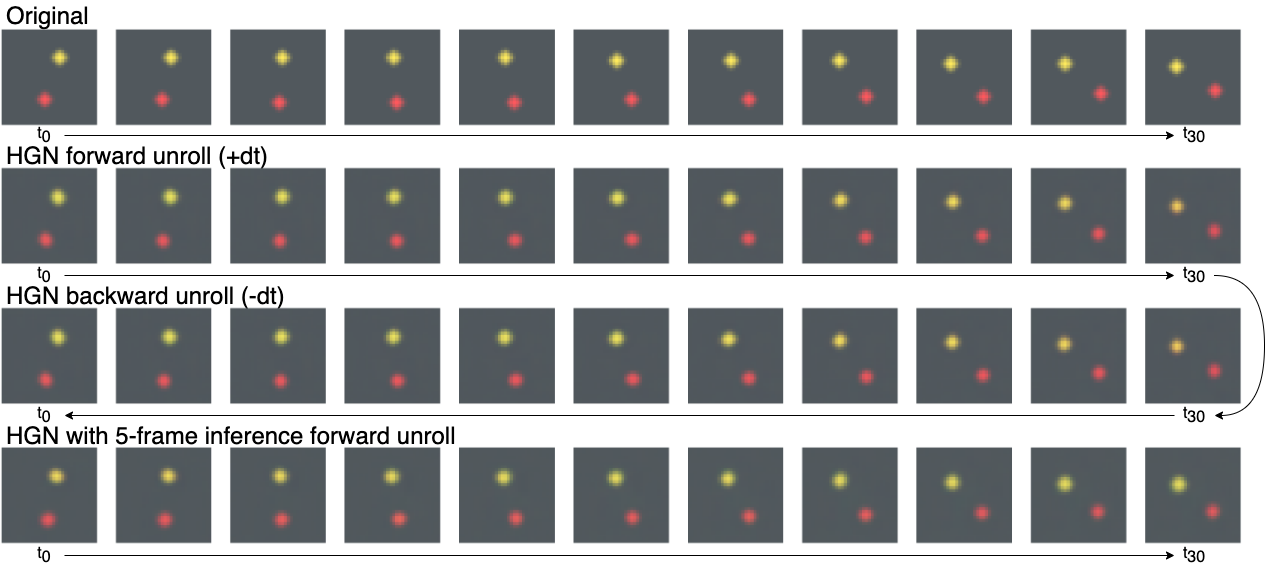
\includegraphics[width=.9\linewidth]{../openreview/pictures/rollout_samples/new_forward_unroll_2_body.png}
        \label{fig:rollout-3-body}
        \caption{}
    \end{subfigure}
    \begin{subfigure}{.48\textwidth}
        \centering
        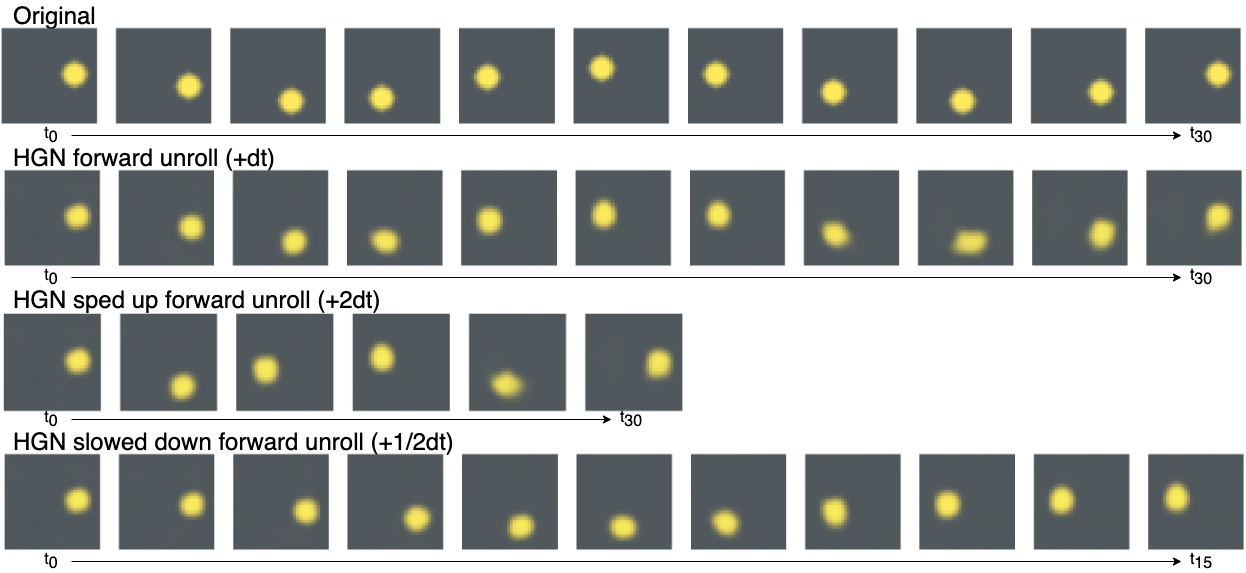
\includegraphics[width=.9\linewidth]{../openreview/pictures/rollout_samples/new_forward_backward_unroll_pendulum.png}
        \caption{}
        \label{fig:rollout-pendulum}
    \end{subfigure}
    \caption{(a) Reconstruction of a sequence of the 2-body system along with a backward unroll of the data from the final state, and a forward rollout of the HGN trained using state inference from the first 5 frames. (b) Reconstruction of a sequence of the pendulum system along with a sped up and a slowed down forward rollout.}
    \label{fig:rollout_back_forth}
\end{figure}

In Figure \ref{fig:rollout_back_forth}, we show some qualitative examples of the reconstructions obtained by the full version of HGN. The model can reconstruct the samples and its rollouts can be reversed in time, sped up, or slowed down by changing the value of the time step used in the integrator. Since the HGN is designed as a generative model, we can sample from the latent space to produce initial conditions and perform their time evolution. We show some rollouts obtained this way in figure \ref{fig:samples}. We observe that our model is only able to generate plausible and diverse samples in the mass-spring dataset.
This behavior is different than the one shown by \cite{hgn} and might be caused by different hyper-parameter configurations in the training procedure or some implementation mistake.
% Later discussion with the authors revealed that they did not input the whole rollout to the encoder but just the first five frames, which was not explained in the paper. Since we received the information too late, we could not run all the experiments again.
% However, we tried this modification in the \textit{mass-spring} dataset, achieving a reconstruction loss of $1.4\times 10^{-3}$, which is very similar to authors results. 


% - The way we assess error: larger bodies with more movement gets more penalized
% - 2-3 bodies move slower and seems better for our model
% - Seems that our hyper-parameter choice is better at physics and theirs better at reconstruction
% - Identify good/bad physiscs and good/bad reconstructions


% Below we comment on the results reported for each environment.

% We takl about mass spring. then talk about pendulum. 
We achieve slightly larger MSE in the autoencode version and significantly larger in the 5-frame inference problem on both the mass-spring and pendulum.
The latter presents roughly double MSE probably because of a wider span of movement.
In general, these two environments show worse results in comparison to two/three-bodies.
For these last cases, our implementation using the \textit{autoencode} setting outperforms the original HGN \cite{hgn}, and when using the \textit{5-frame inference} the results are similar.
As we can see, these two environments show much less average pixel MSE compared to the first ones (almost one order of magnitude).
We believe this may be due to the differences when rendering the instances of each dataset.
The elements appearing in mass-spring and pendulum (represented by a large yellow ball) are larger than the ones present in the two/three bodies (two/three small coloured balls).
Because of this, it would be reasonable to assume that localization errors are more penalized in the first two environments, since the total difference in areas is larger.
Furthermore, the dynamics representing mass-spring and pendulum show faster movements in comparison to two/three-bodies, resulting in being harder to represent with our HGN.
Consequently, we hypothesise the following: larger elements and faster dynamics, produces higher average MSE on our model regardless of the difficulty of the environment physics.
However, this is not the case for the original author's results, who seem to struggle more on the two/three-bodies.
Surprisingly, it seems that our hyperparameter and architecture choices led to poorer reconstruction capabilities (higher MSE) but learning better physics (qualitatively more realistic movements).
% The error gets severely exacerbated when only inputting the first 5 frames of the sequence.

% In fact, 2 bodies are tal tal ,3 bodies are tal tal, and it is because of the previous assumption.






% \begin{itemize}
%     \item \textbf{Mass-spring and Pendulum:}

    
%     In comparison, both environments seem to be harder for us to learn than the multiple bodies ones.
     
%     % Surprisingly, it seems that our hyperparameter and architecture choices let to learning better physics but poorer reconstruction capabilities.

%     \item \textbf{Two-body and Three-body:} As we observe, our implementation using the \textit{autoencode} setting is able to outperform the original HGN \cite{hgn}. On the other hand, when using \textit{5-frame inference}, the results are still comparable. 
    
%     %Although it is hard to draw an exact conclusion on the factors causing these results, we can see the instances represented in the \textit{two/three-body} dataset are smaller compared to the ones in the \textit{mass-spring} or \textit{pendulum} (see Figure \ref{fig:datasets} for reference). Moreover, the dynamics of the \textit{two/three-body} systems are steadier. These two factors
    
%     Autoencode is better than them, 5-frames is similar
%     \item \textbf{Three-body:} Both autoencode and 5-frame better than them. Why?
% \end{itemize}


\begin{figure}
    \centering
    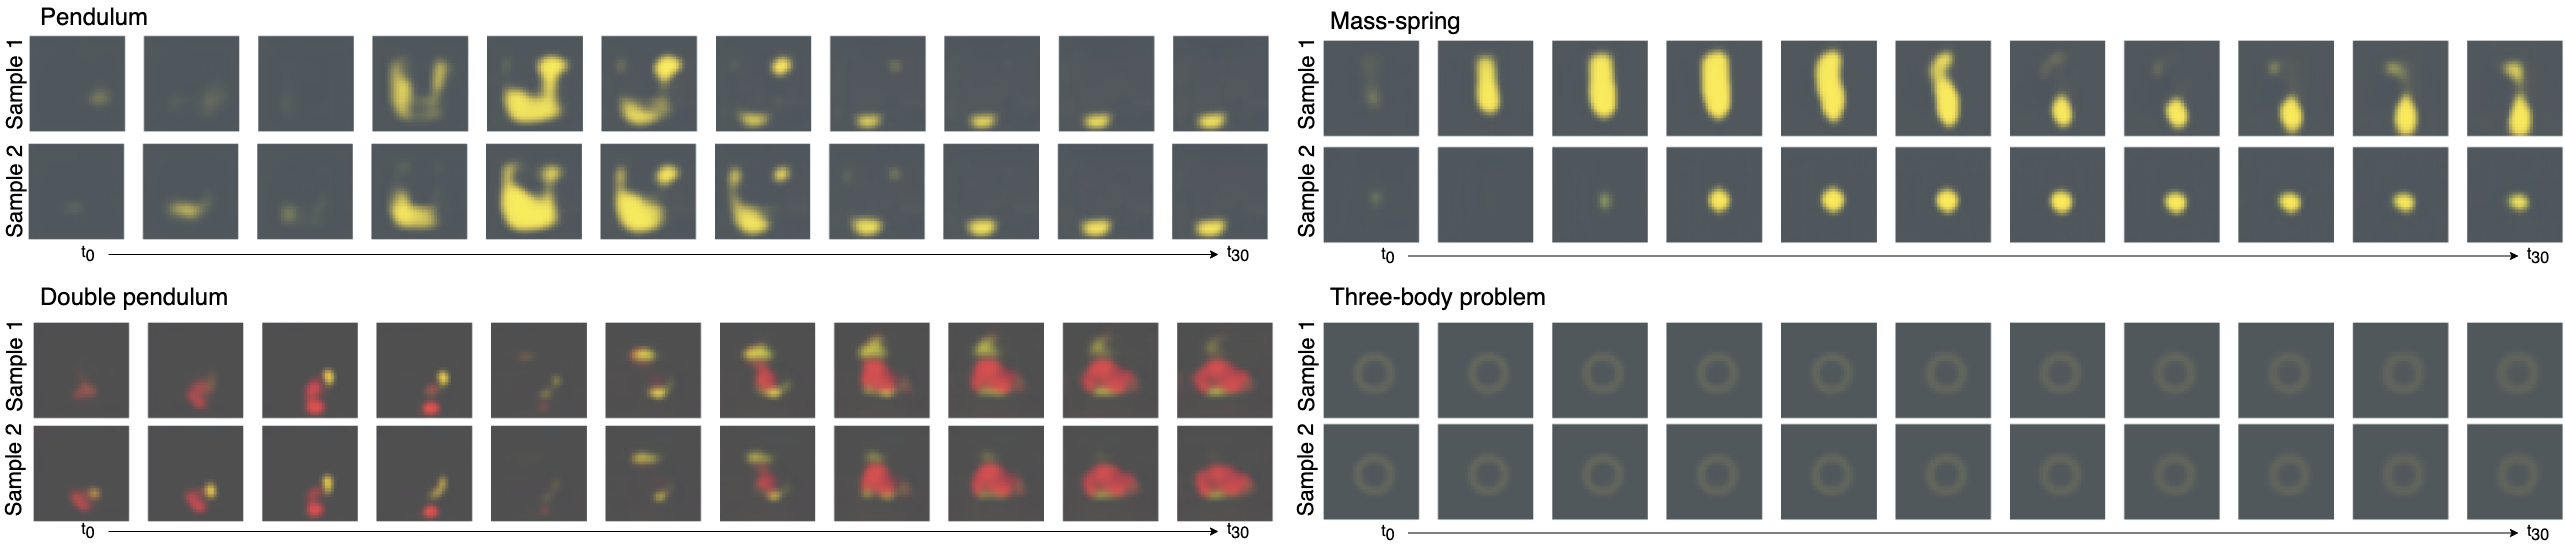
\includegraphics[width=\textwidth]{../openreview/pictures/rollout_samples/new_sampling.png}
    \caption{Examples of sample rollouts from the latent space for different physical systems.}
    \label{fig:samples}
\end{figure}

\subsection{Additional experiments} \label{sec:additional_experiments}

\paragraph{GECO parameter search} \label{sec:hyperparam_search} The paper does not provide the values of GECO \cite{geco} used. In GECO, the Lagrangian multiplier is optimized at each step with a rate $\gamma$.
Figure \ref{fig:geco_search} shows the behavior of GECO for $\gamma \in \{0.1, 0.05, 0.01\}$ in terms of reconstruction loss and KL divergence. Higher values of $\beta$ give a better reconstruction loss but greatly increase the KL divergence. %In our experiments we generally use $\beta = 0.05$, which provides a good trade-off, or $\beta = 0.1$ for environments in which reconstruction is harder (e.g. pendulum).
However, we found that hyperparameters were not consistent among different environments and integrators. For this reason, we do not use GECO in our experiments.
\begin{figure}[]
\minipage{0.5\textwidth}
\centering
  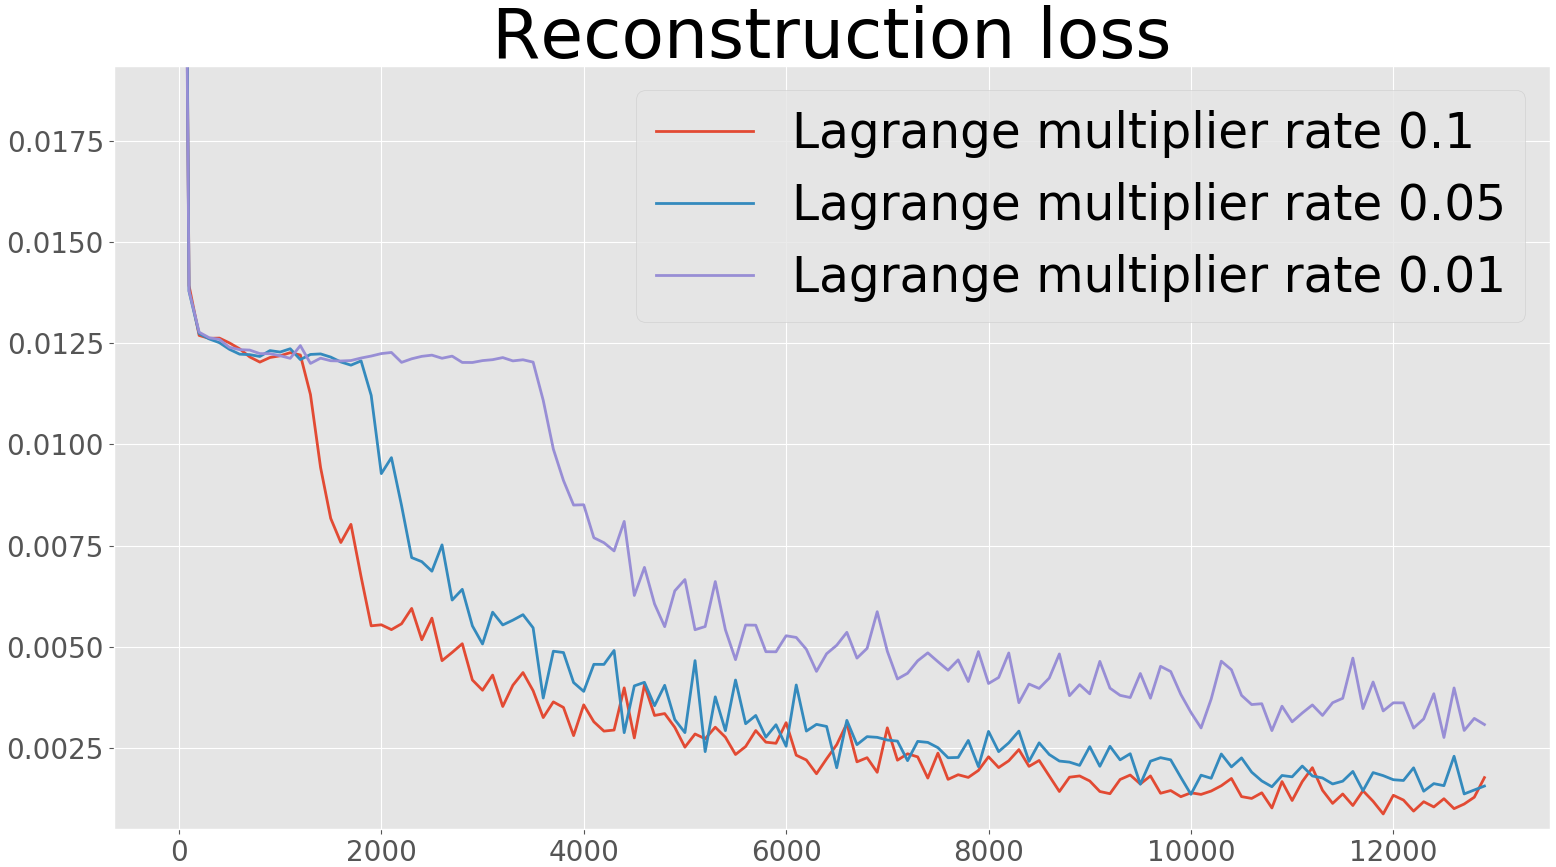
\includegraphics[width=0.8\linewidth]{../openreview/pictures/parameter_comparisons/lagrange_multiplier_comparison_rec_loss.png}
\endminipage\hfill
\minipage{0.5\textwidth}
\centering
  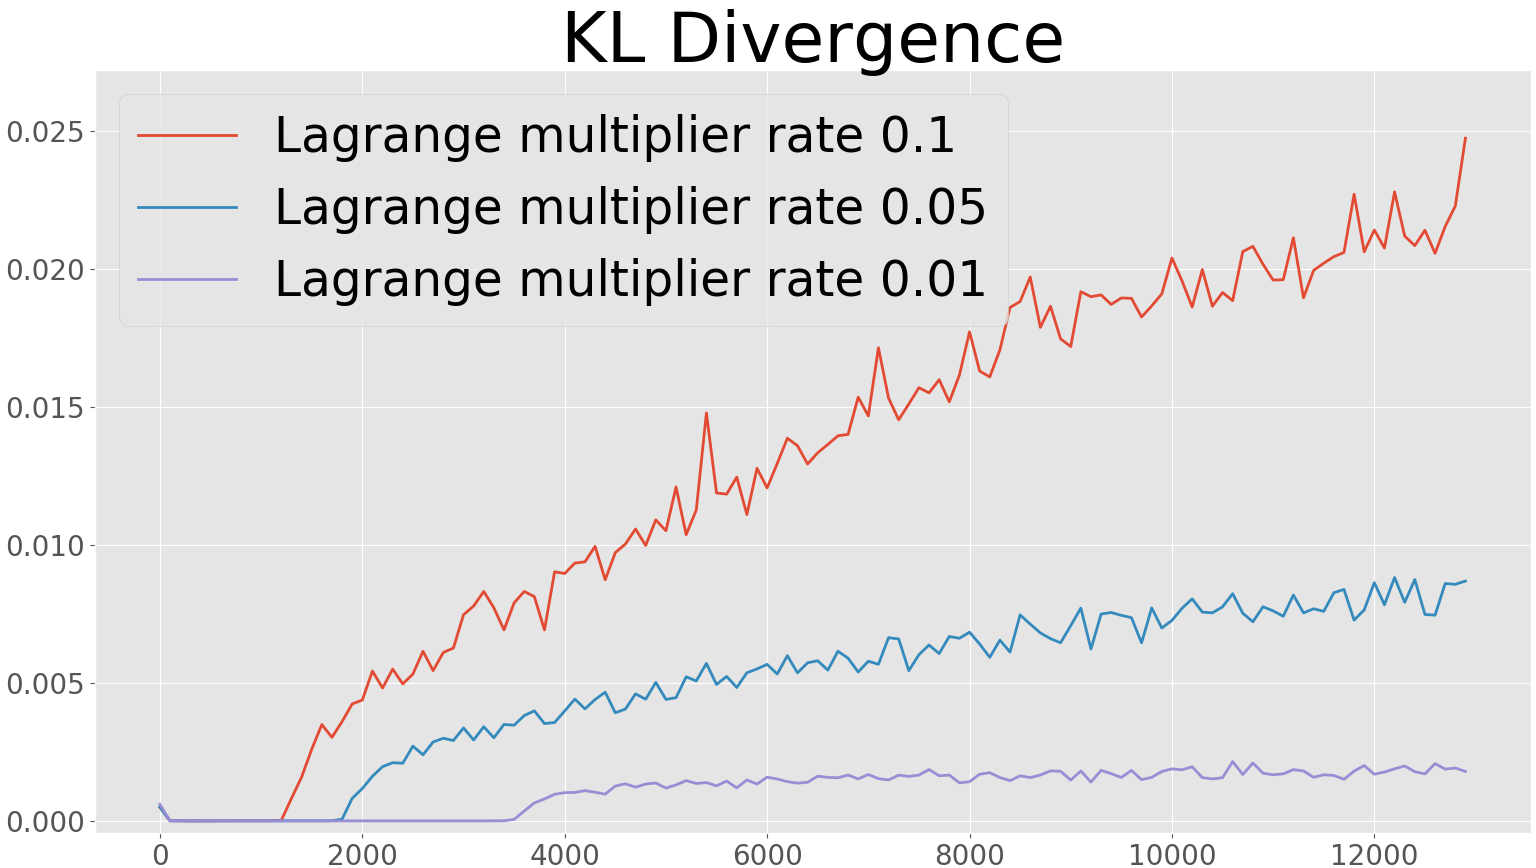
\includegraphics[width=0.8\linewidth]{../openreview/pictures/parameter_comparisons/lagrange_multiplier_comparison_kld.png}
\endminipage
\caption{Reconstruction loss and KL divergence for different GECO parameters in the Pendulum environment.}
\label{fig:geco_search}
\end{figure}


\paragraph{Integrators} \label{sec:integrators}
Performing the integration step is key to generate the time evolution of a rollout given the initial state. 
In the HGN paper \cite{hgn} the system is tested using Euler and Leapfrog integration. We wonder if using higher order integration methods might boost the performance of the rollout generation process.
% The Runge-Kutta integration is only used when training the HNN architecture \cite{hnn}. 
%We observed that one main disadvantage of Euler integration is that its errors accumulate rapidly over longer time periods.
Therefore, we implement and test the HGN architecture with two additional numerical integration methods: the Runge-Kutta's 4th-order integrator \cite{rk4} and the 4th-order Leapfrog integrator (Yoshida's algorithm \cite{yoshida1992symplectic}). Table \ref{tab:integrators} shows a comparison of all four integrators on the Pendulum dataset.
%For this reason other methods that involve more integration steps, such as the fourth-order Runge-Kutta integration (RK4) or the fourth-order Leapfrog (Yoshida's algorithm) \cite{yoshida1992symplectic} have been implemented.
Both Leapfrog and Yoshida are \textit{symplectic} integrators: they guarantee to preserve the special form of the Hamiltonian over time \cite{neal2011mcmc}.
% , at the cost of slower execution.

\begin{table}[]
    \centering

    \begin{tabular}{c c c c c}
     \Xhline{3\arrayrulewidth}
      & \textsc{Euler} & \textsc{Runge-kuta 4} & \textsc{Leapfrog} & \textsc{Yoshida}\\

     \Xhline{3\arrayrulewidth}
     pixel MSE & $17.86 \pm 0.13$ & $76.88 \pm 0.08$ & $14.97\pm 0.10$ & $14.70\pm 0.10$ \\
     $\mathcal{H}$ std & $3.81$ & $0$ & $1961.93$ & $1893.05$\\
     reconstr. time (s) & $0.32$ & $1.89$ & $0.96$ & $1.61$ \\

     \Xhline{3\arrayrulewidth}
    
    \end{tabular}
    \vspace{0.25cm}
    \caption{Comparison between four different integrators used to perform the time evolution in the HGN. The results are measured on the simple pendulum test set. The pixel MSE values have been multiplied by $10^4$.}
    \label{tab:integrators}
\end{table}

Table \ref{tab:integrators} shows the average pixel MSE, the averaged standard deviation of the output of the Hamiltonian network during testing, and the reconstruction time of a single batch ($\texttt{batch}=16$) using the different integration methods that we have described previously. The model has been trained on the simple pendulum dataset. As we can see, the reconstruction time increases when using higher-order integration methods, since they require more integration steps. In general, we see that Euler integration offers a fast and sufficiently reliable reconstruction of the rollouts. Moreover, we observe that the fourth-order symplectic integrator (Yoshida) achieves the best performance. Surprisingly, the symplectic integration methods show more variance in the output of the Hamiltonian networks throughout a single rollout. This behavior is unexpected since using a symplectic integration method should ideally keep the value of the Hamiltonian invariant. We conclude that more experiments need to be performed to guarantee that the implementation of both Leapfrog and Yoshida integration methods are faithful to their formulation.


\paragraph{Integrator modelling} We train the modified architecture of Section \ref{sec:integrator_modelling} on the Pendulum dataset for 5 epochs. The architecture is the same as HGN, but the Hamiltonian Network now outputs $\Delta q$ and $\Delta p$. The average MSE error over the whole Pendulum dataset is $1.485\times 10^{-3}$, while in the test set it is $1.493 \times 10^{-3}$, which are both very close ($\sim \pm 2\%$) to those of autoencoding HGN (see Table \ref{tab:reproduction}). The modified architecture is still capable of performing forward slow-motion rollouts by modifying $\Delta t$. We set $\Delta t' = \frac{\Delta t}{2}$ and we compute the average MSE of the slow-motion reconstruction over 100 rollouts. The modified architecture achieved an error of $8$x$10^{-4}$, while the standard HGN achieved $9$x$10^{-4}$. Note that reconstruction losses are smaller for slow-motion as the images change less between timesteps.



\paragraph{Extra environments}
Apart from the four physical systems presented by \cite{hgn} we test our re-implementation of the HGN with physical systems that do not have a simple Hamiltonian expression. As described previously, these are the damped harmonic oscillator and the double pendulum. On one hand, we are interested in a damped system since it introduces a dissipative term to the equations of motion; a feature that differs from the previous systems. On the other hand, the double pendulum is modelled by a non separable Hamiltonian: $\mathcal{H}(\textbf{q},\textbf{p}) \neq K(\textbf{p}) + V(\textbf{q})$ as described previously. In figure \ref{fig:extra} we show some visual examples of the reconstructions provided by the HGN trained on the two systems. As we can see, HGN is able to reconstruct the damped oscillator with high reliability. Regarding the double pendulum, we observe that the model reconstructs well small oscillations, but fails when the trajectory is too chaotic as expected. The average pixel MSE of the reconstructions of the damped oscillator and the double pendulum are $6.39\cdot 10^{-4}$ and $6.91\cdot 10^{-4}$ respectively. The HGN is able to provide better reconstructions for these systems in comparison to the mass-spring and pendulum systems.

\begin{figure}
    \centering
        \begin{subfigure}{.48\textwidth}
        \centering
        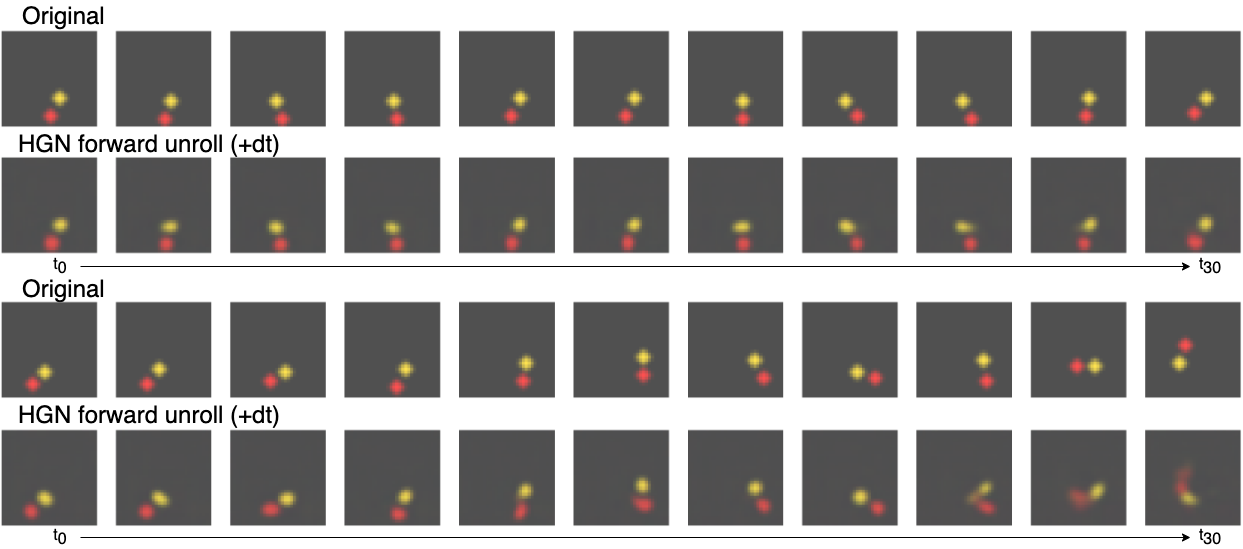
\includegraphics[width=\linewidth]{../openreview/pictures/rollout_samples/new_chaotic_pendulum_rollouts.png}
        \label{fig:a}
    \end{subfigure}
    \begin{subfigure}{.48\textwidth}
        \centering
        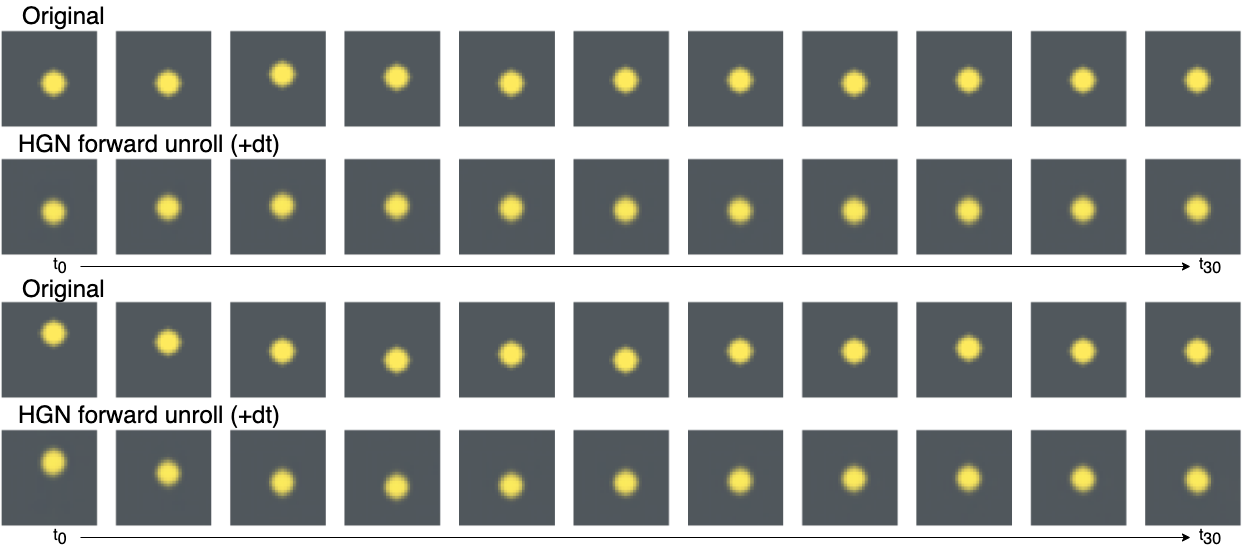
\includegraphics[width=\linewidth]{../openreview/pictures/rollout_samples/new_damped_spring_sample_rollout.png}
        \label{fig:b}
    \end{subfigure}
    \caption{Examples of reconstructions of the double pendulum (left) and the damped harmonic oscillator (right).}
    \label{fig:extra}
\end{figure}


\section{Discussion}
\label{sec:disc}
% Give your judgement on if you feel the evidence you got from running the code supports the claims of the paper. Discuss the strengths and weaknesses of your approach - perhaps you didn't have time to run all the experiments, or perhaps you did additional experiments that further strengthened the claims in the paper.

% Summary
We were able to implement and train an Hamiltonian Generative Network with similar reconstruction performance of the ones of the original paper  ($30\%$ average absolute relative error wrt to their reported values when treating it as an autoencoder). These results show that the network is capable of exploiting the Hamiltonian equations to learn dynamics of a physical system from RGB images. However, the value of the resulting Hamiltonian does not remain constant throughout the system evolution. 
% \todo{Carles, Oleguer, check that what I write here makes sense}
This means that the network is learning something that is different from the Hamiltonian equations described in Section \ref{sec:data}.
%It is worth to note that there is an infinite number of equations whose partial derivatives in $q$ and $p$ match those of Eq. \ref{eq:hamilton}. In particular, a constant could be added to all Hamiltonian equations of Section \ref{sec:data} without changing the derivatives used by the integrators. Therefore, at each time-step the Hamiltonian network could predict any of these equations, explaining the high variance in the Hamiltonian values.   

To make the variational sampling work, we tried performing a grid search on the Geco\cite{geco} hyperparameters and using a fixed Lagrange multiplier as in \cite{beta-vae}. However, despite our best efforts, the samples produced by the variational model have very poor quality. This is generally due to the difficulty in minimizing both KL divergence and reconstruction loss. 

%To better evaluate the system, we provided further experiments giving a better grasp of the possibilities the Hamiltonian paradigm opens when using ANNs to learn about dynamical systems.
% Future work
We believe that further experiments are needed to understand better the behavior of the system and to improve it. Future work could include further testing on each network architecture, probably smaller networks would also be able to encode the needed information. Another next step is to try the approach on more challenging (and realistic-looking) environments. In addition, it would be interesting to tackle the transfer learning capabilities of such architecture between different environments. How re-usable each network is? How much faster the system is able to learn the new dynamics? Finally, another field which could benefit from this research is model-based reinforcement learning.
A generative approach from which to sample example rollouts could be very useful for training agents without the need of directly interacting with the environment.

\subsection{What was easy}
% Give your judgement of what was easy to reproduce. Perhaps the author's code is clearly written and easy to run, so it was easy to verify the majority of original claims. Or, the explanation in the paper was really easy to follow and put into code. 

% Be careful not to give sweeping generalizations. Something that is easy for you might be difficult to others. Put what was easy in context and explain why it was easy (e.g. code had extensive API documentation and a lot of examples that matched experiments in papers). 
Once we implemented the code it resulted quite easy to perform multiple experiments on different environments, architectures and hyper-parameters due to the code's modularity and flexibility.
We can define the the previously mentioned experiments and most common testing behaviors from a set of yaml files which can then be modified from command-line arguments.
While this required extra planning and work at the beginning it really payed off when debugging and evaluating in later stages. 

\subsection{What was difficult} \label{sec:challenge}
% List part of the reproduction study that took more time than you anticipated or you felt were difficult. 

% Be careful to put your discussion in context. For example, don't say "the maths was difficult to follow", say "the math requires advanced knowledge of calculus to follow". 

The main challenge we encountered is finding the correct tools to debug a model composed of so many interconnected networks.
The fact that it has a variational component with a dynamic Lagrange multiplier term makes it especially tricky to train.
Furthermore, no public implementation existed and some details and parameters were missing in the original paper leading to some necessary assumptions or parameter searches.


\subsection{Communication with original authors}
% Document the extent of (or lack of) communication with the original authors. To make sure the reproducibility report is a fair assessment of the original research we recommend getting in touch with the original authors. You can ask authors specific questions, or if you don't have any questions you can send them the full report to get their feedback before it gets published. 
We first tried to understand and re-implement the code by ourselves.
Nevertheless, at some point we had gathered a significant set of doubts and we decided to email them to the original authors, which they answered with great detail.
From that point onwards, we sent a couple more set of doubts, also receiving answers.\\

Most of our doubts were about network architecture clarifications (either of unclear or missing descriptions from the original paper), and loss function evaluation.
Furthermore, they provided us with some of their environment images so we could more easily make our environments as similar as possible.

\subsection{Improving reproducibility}
Having worked in re-implementing the whole original work, we feel it is important to share our experience as well as providing a recommendation on how it could be made more easily reproducible.
First, having the environments data or code to generate it available online would save the effort and, most importantly, it would constitute a baseline against which to compare future work.
Secondly, publishing all the hyperparameters and more details of the networks architecture would make the whole work much easier to reproduce and require less training attempts, especially for what concerns GECO.


\section*{Acknowledgements}
We thank Stathi Fotiadis for voluntarily contributing with a GECO \cite{geco} implementation draft to the public \href{https://github.com/CampusAI/Hamiltonian-Generative-Networks}{repo} and his useful feedback on code structuring. We thank the KTH Robotics, Perception, and Learning (RPL) Lab for the computational resources provided to us.
In addition, we would like to thank the original authors for providing further details on the implementation.
